\documentclass[a4paper]{article}
\usepackage[utf8x]{inputenc}
\usepackage[english]{babel}

\usepackage[margin=2cm]{geometry}
\usepackage{amsmath}
\usepackage{multicol}
\usepackage{nicefrac}
\usepackage[rflt]{floatflt}



\pagestyle{empty}



\usepackage{tikz}
\usetikzlibrary{calc, intersections}


\begin{document}

\def\aalpha{20}
\def\pphi{30}
% \newcommand\vv[1]{\overrightarrow{#1}}

\section*{CAR MOVEMENT}
Along this project, consider \textbf{counterclockwise} angles to be positives. Besides, the rendered car will use Front Wheel Drive (from now FWD).

% \begin{multicols}{2}

	\begin{floatingfigure}{0.55\textwidth}
		\setlength\unitlength{2cm}
	\begin{tikzpicture}[x=1\unitlength,y=1\unitlength]
		\node[opacity=0.4, inner sep=0mm] (CAR) {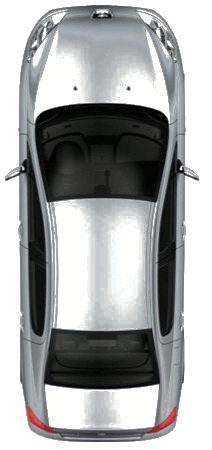
\includegraphics
					[width=1\unitlength,height=2\unitlength]{../car2.png}};

		\draw[opacity = 0.3, thick, -to] ($(CAR.south) +(0,-2mm)$) -- ($(CAR.north) +(0,2mm)$);
		\draw[opacity = 0.3, thick, -to] ($(CAR.west) + (-2mm,0)$) -- ($(CAR.east) + (2mm,0)$);

		% INTERAXIS LENGTH
		\draw[thick, dashed] ($(CAR.north east) + (-0.13,-0.4\unitlength)$) -- +(0.4,0) coordinate (IAL1);
		\draw[thick, dashed] ($(CAR.south east) + (-0.13,0.4\unitlength)$) -- +(0.4,0) coordinate (IAL2);
		\draw[thick, to-to] ($(IAL1.center) - (2mm,0)$) --
			node[right] {\small $D$}
			($(IAL2.center) - (2mm,0)$);

		% CAR LENGTH
		\draw[thick, dashed] ($(CAR.north east) + (-0.5,-0.03\unitlength)$) -- +(1,0) coordinate (L1);
		\draw[thick, dashed] ($(CAR.south east) + (-0.5,0.03\unitlength)$) -- +(1,0) coordinate (L2);
		\draw[thick, to-to] ($(L1.center) - (2mm,0)$) --
			node[right] {\small $L$}
			($(L2.center) - (2mm,0)$);

		% CAR WIDTH
		\draw[thick, dashed] ($(CAR.west) + (+0.09\unitlength, 0)$) -- +(0, -1.2) coordinate (W1);
		\draw[thick, dashed] ($(CAR.east) + (-0.13\unitlength, 0)$) -- +(0, -1.2) coordinate (W2);
		\draw[thick, to-to] ($(W1.center) + (0,2mm)$) --
			node[below] {\small $W$}
			($(W2.center) + (0,2mm)$);

		\begin{scope}[shift={(2.5,0)}]
			\draw[thick] (0,-1.2) -- (0,1.4);
			\draw[thick, -to] (0,0.5) arc (90:90+\aalpha:0.5)  node[midway, above] {\small $\alpha$};
			\begin{scope}[rotate=\aalpha]
				\node[rotate=\aalpha, opacity=0.4, inner sep=0mm] (CAR2) {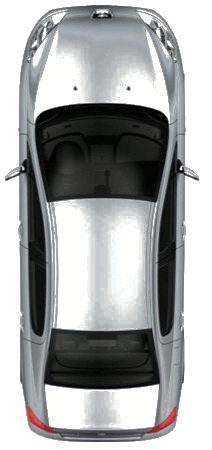
\includegraphics
							[width=1\unitlength,height=2\unitlength]{../car2.png}};
				\draw[thick, -to] ($(CAR2.south) +(0,-2mm)$) -- ($(CAR2.north) +(0,6mm)$);
				% WHEELS
				\begin{scope}[shift={($(CAR2.north west) + (0.11,-0.4\unitlength)$)}]
					\draw[rotate=\pphi, very thick] (0,-0.07) -- (0,0.07);
					\draw[rotate=\pphi] (0,0) -- (0,0.4);
					\draw[] (0,-0.4) -- (0,0.4);
					\draw[thick, -to] (0,0.2) arc (90:90+\pphi:0.2) node[midway,above left=-1mm] {\small $\varphi$};
				\end{scope}


			\end{scope}
			\begin{scope}[shift={(-0.8,-0.6)}]
				\draw[-to] (-0.3,0) -- ++(0.6,0);
				\draw[-to] (0,-0.3) -- ++(0,0.6);
				\node[below right]{\small $(0,0)$};
				\draw[thick, -to] (0,0) -- node[left] {\small $\mathbf{x}$} (CAR2.center);
			\end{scope}
		\end{scope}

	\end{tikzpicture}
	\end{floatingfigure}
	~
	\begin{itemize}
  	\setlength\itemsep{-1em}
		\fltitem{$L$: Car Length.}
		\fltitem{$W$: Car Width.}
		\fltitem{$D$: Interaxis Length.}
		\fltitem{$\alpha$: Car orientation.}
		\fltitem{$\varphi$: Steering wheel angle.}
		\fltitem{$\Delta t$: Elapsed time.}
		\fltitem{$\mathbf{x}$: Position of the car.}
		\fltitem{$\Delta \theta$: Increment on car orientation.}
		\fltitem{$\Delta \mathbf{x}$: Increment on car position.}
		\fltitem{$v$: Car velocity. Measured as average of front wheel velocities.}
	\end{itemize}


\def\pphi{-30}
\def\aalpha{10}
\setlength\unitlength{2cm}
	\begin{floatingfigure}{0.4\textwidth}
	\begin{tikzpicture}[x=1\unitlength,y=1\unitlength]
		\node[rotate=\aalpha, opacity=0.4, inner sep=0]
				(CAR) {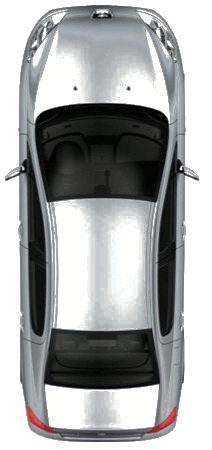
\includegraphics [width=1.0\unitlength, height=2.0\unitlength]{../car2.png}};
		 \coordinate (REAR) at ($(CAR.center)!0.65!(CAR.south)$);
		 \coordinate (FRONT) at ($(CAR.center)!0.65!(CAR.north)$);

		 \node[left] {\small $C$};
		 \node[left] at (FRONT) {\small $F$};
		 \node[left] at (REAR) {\small $R$};


		\draw (REAR) -- +(2\unitlength,0);

		% ROTATION ANGLE
		\begin{scope}[shift={(REAR)}]
			\draw[thick, -to] (0.7,0) arc (0:\aalpha:0.7) node[midway, right] {\small $\alpha$};
			\draw[rotate=\aalpha] (0.1,0) -- ++(0,0.1) -- ++(-0.1,0);
		\end{scope}

		\begin{scope}[rotate=\aalpha]
			\draw[thick] ($(CAR.south) + (0,-.05\unitlength)$)
			-- ($(CAR.north) + (0,.05\unitlength)$);
			% WHEEL
			\begin{scope}[shift={(FRONT)}]
				\draw[rotate=\pphi, very thick] (0,-0.07) -- (0,0.07);
				\draw[rotate=\pphi] (0,0) -- (0,0.4);
				\draw[thick, -to] (0,0.2) arc (90:90+\pphi:0.2) node[midway,above = 2mm, right=-2mm] {\small $\varphi$};
			\end{scope}

			% REAR WHEEL RADIUS
			\path[name path = rearpath] (REAR) -- +(2.5\unitlength,0);
			% FRONT WHEEL RADIUS
			\path[name path = frontpath] (FRONT) -- +(\pphi:2.7\unitlength);
			\path[name intersections={of=rearpath and frontpath, by=O}];
			\node[right] at (O) {\small $O$};
			\draw[thick] (FRONT) -- node[above] {\small $R_F$} (O);
			\draw[thick] (REAR) -- node[above=1mm, left=2mm]{\small $R_R$} (O);
			\draw[thick] (CAR.south) -- node[below] {\small $R_T$} (O);
			\draw[thick, name path = centerpath] (CAR.center) -- node[above] {\small $R_C$} (O);

			% PHI and BETA ANGLES
			\begin{scope}[shift = {(O)}]
				\draw[thick,-to] (-0.8,0) arc (180:{180+atan(tan(\pphi)/2)}:0.8) node[midway,left] {\small$\beta$};

				\draw[thick,-to] (-0.4,0) arc (180:{180+\pphi}:0.4) node[midway,left=0.5mm,fill=white,inner sep=0] {\small$\varphi$};

			\end{scope}

			\draw[very thick, -to] (0,0) -- ($(0,0)!8mm!(O)$) coordinate (AA);
				\node[above] at (AA) {\small $\vec{a}$};


			\path (AA) arc ({atan(tan(\pphi)/2)}:90+atan(tan(\pphi)/2):8mm) coordinate (BB);

			\draw[very thick, -to] (0,0) -- (BB);
				\node[right] at (BB) {\small $\vec{b}$};
		\end{scope}

	\end{tikzpicture}\end{floatingfigure}

	Supose the car orientation to be $\alpha >0$ (according to picture) wheels angle to be $\varphi < 0$. The car turns around point $O$ with radius $R_F$ of front wheel axis, $R_C$ to the center of the car (the position of the car) and $R_R$ to the rear wheel axis.
	\[
		\boxed{R_F = \frac{D}{\sin(\phi)}}
	\]
	\[
		\tan\beta = \frac{D}{2\,R_R},\quad tan\varphi = \frac{D}{R_R} \Longrightarrow
		\boxed{\beta = \arctan\left(\frac{\tan\varphi}{2}\right)} \in [-\nicefrac\pi2,\nicefrac\pi 2]
	\]
	\[
	\boxed{R_C = \frac{D}{2\sin\beta}}
	\]

	$\vec{a}$ and $\vec{b}$ are the vectors of the canonical base rotated $\alpha + \beta$:
	\[
	\begin{split}
		\vec{a} &= \cos (\alpha+\beta) \vec{\i} + \sin(\alpha+\beta) \vec{\j}\\
		\vec{b} &= -\sin (\alpha+\beta) \vec{\i} + \cos(\alpha+\beta) \vec{\j}
	\end{split}
	\]

	From velocity of front wheels we can compute the angular velocity and the increment $\Delta \theta$ on car rotation in $\Delta t$:
	\[
	\boxed{\omega = \frac{v}{R_F}} \Longrightarrow
	\boxed{\Delta \theta = \frac{v\cdot\sin(\varphi)\cdot\Delta t}{D}}
	\]


	\setlength\unitlength{2cm}
	\def\dt{40}
	\begin{floatingfigure}{0.4\textwidth}
		\begin{tikzpicture}[x=1\unitlength,y=1\unitlength]
			\draw[very thick, -to] (0,0) -- (0.5,0) coordinate (AA);
			\draw[very thick, -to] (0,0) -- (0,0.5) coordinate (BB);
			\node[below left] {\small $C$};

			\node[above] at (AA) {$\small \vec{a}$};
			\node[left] at (BB) {$\small \vec{b}$};

			\draw[thick] (0,0) arc (180:{180-\dt}:1.5);

			\begin{scope}[shift={(1.5,0)}]
				\node[below right] {\small $O$};
				\draw (0,0) -- node[below] {\small $R_C$} (-1.5,0);
				\draw (0,0) -- ({180-\dt}:1.5);
				\draw[thick,-to] (-0.5,0) arc (180:{180-\dt}:0.5)
					node[midway, left] {\small $\Delta \theta$};
				\draw[thick,-to] (-1.5,0) --
				 	node[right] {\small $\Delta \mathbf{x}$} ($(-1.5,0)!0.98!({180-\dt}:1.5)$);
			\end{scope}
		\end{tikzpicture}
	\end{floatingfigure}

	And the displacement of the center can be computed in terms of $\vec{a}$ and $\vec{b}$:
	\[
	\Delta \mathbf{x} = R_C (\cos(\Delta\theta)-1) \vec{a} + R_C\sin(\Delta\theta) \vec{b}.
	\]
	And we have the final equations for $\delta x$ and $\Delta y$:
	\[
	\boxed{\begin{split}
		\Delta x &= R_C (\cos(\Delta\theta)-1) \cos(\alpha + \beta) - R_C \sin(\Delta\theta) \sin(\alpha+\beta),\\
		\Delta y &= R_C (\cos(\Delta\theta)-1) \sin(\alpha + \beta) + R_C \sin(\Delta\theta) \cos(\alpha+\beta).
	\end{split}}
	\]


\end{document}
